\documentclass{article}
\usepackage[utf8]{inputenc}
\usepackage{graphicx}
\usepackage{hyperref}
\usepackage{pgfplotstable}
\usepackage{geometry}
\geometry{
 a4paper,
 left=30mm,
 right=30mm,
 top=20mm,
 bottom=20mm
}


\title{EECS 447 Course Project: Goop}
\author{Zai Erb, Nicholas Nguyen, Chinh Nguyen}
\date{}

\begin{document}

\maketitle

\tableofcontents

\newpage

\section{Introduction}

\quad \quad Goop is an application that allows users to view, save, share, and find songs, albums, DJ Mixes, and artists. 
Its primary feature is its fine-tuned searching and cataloging of music based on any user-given parameters. 
The database allows users to see specific information about music such as release date, record label, performing artists, DJ mixes, and more. 
For example, if a user wants to display every DJ mix that contains a specific song or artist 
or if they want to see a record label's discography from a specified timeframe. 

Each user account with their profiles and account information are stored in the database. 
Additionally, users are able to save and organize their music. Users are allowed to follow each other in addition to artists, labels, genres. 
This service is primarily useful for DJs/performers who are "crate digging" or finding new music to play in their mixes. 
Being able to fine-tune search results based on adjacent information (such as which mixes a song was played in or the labels an artist is on) 
in a collection will assist in organizing record libraries in external applications like Rekordbox, Serato, or VirtualDJ. 

The concept for Goop was born from frustrations we have had with the existing options for music cataloging. 
There are lots of options but all of them have significant drawbacks, the biggest of which is that they all have a narrow scope, designed to focus on 
one specific aspect of music cataloging and categorization, the other issue that is ubiquitous with these sites is a severely outdated, often hard to navigate UI. 
Rate Your Music and Album of the Year exist for rating, reviewing, and cataloging tracks and albums but neither of them provide tracklists for DJ mixes and while
Rate Your Music has more data, depth, and flexibility the UI is far worse than the simpler but cleaner Album of the Year site. 
For getting tracklists of DJ mixes there are a few options such as 1001Tracklists, TracklistsDB and Tracklists.net all provide similar functionality
but their interfaces are outdated and the integration of the tracklists with other information such as the album tracks are from, 
their release dates, their associated record labels, the genre of the individual tracks etc. 
For finding events in your area and finding electronic music recommendations Resident Advisor is fantastic 
however it is limited mostly to electronic music and the mixes posted on the site do not have tracklists. 
All of this makes for a frustrating and tedious experience for those that want to dig for music using one platform with a database that connects 
Albums, Genres, Mixes, Labels, Artists, Events and more. 

The biggest challenge for creating an application like this is populating the database. 
A lot of the aforementioned sites rely on community contribution and/or integrate with streaming services such as spotify to ensure new music is added to the database. 
Seeing as implementing solutions like this would not be feasible for our timeline we relied on scraping data from some of these existing sites to test our database schema 
and user interface. If we were to continue with this project we would enable to user contributions and could potentially integrate with streaming services to constantly 
update the database with newly released music.

In this report we will detail what we cover what our app is capable of currently, how it was designed including how we constructed our database and built the front and backend. 
We also cover plans to expand the functionality in the future.

\pagebreak


\section{Design}
    \subsection{SQL} SQL code to create tables and views in database hosted on phpMyAdmin
    \begin{itemize}
        \item SQL used to initialize our tables 
        - $data\_handling/sql/CreateTables.sql$ is the SQL used to initialize our tables
        \item SQL used to initialize views 
        - $data\_handling/sql/CreateViews.sql$ makes querying our database easier especially when there are additional tables
        used to connnect tables such as the Albums table which references the AlbumGenre table which stores album genres and subgenres.
    \end{itemize}

    \subsection{PHP Backend Server} Our backend: $api/akiserver.js$ facillitates interaction with the database, this is where our queries are happening \\ 
    We use the following queries:
    \subsubsection{Queries}
    \begin{itemize} 
        \item Fetching Artists by GenreID:
				\begin{itemize}
					\item 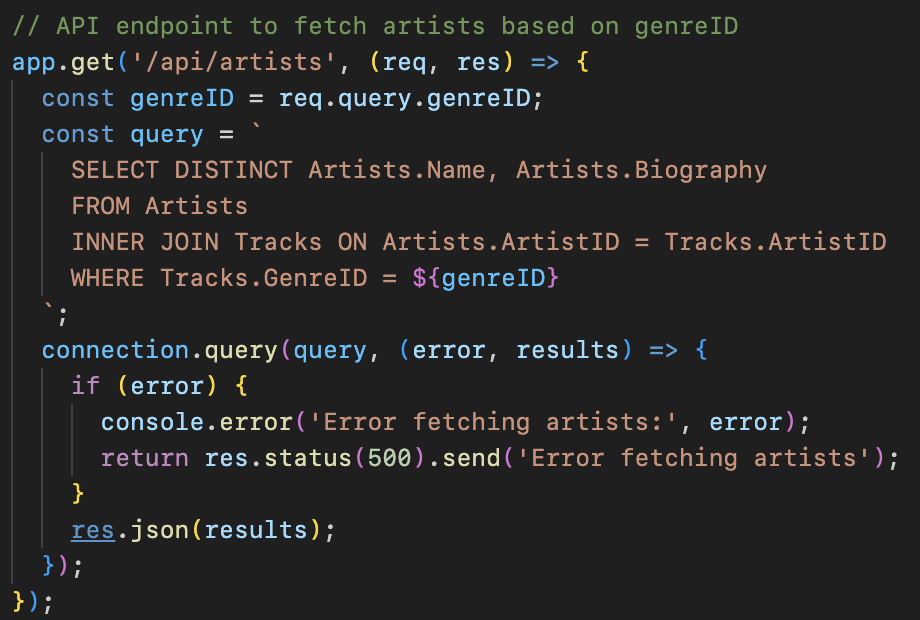
\includegraphics[width=\linewidth]{Queries/fetchArtistsByGenreID.png}
				\end{itemize}
				\item Fetching Albums Information
				\begin{itemize}
					\item 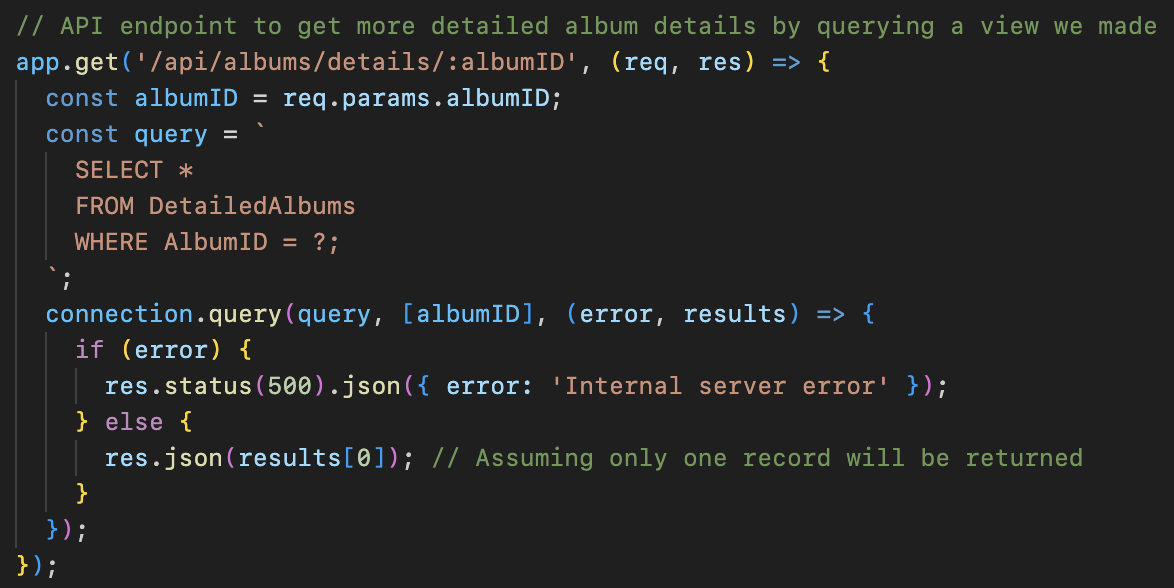
\includegraphics[width=\linewidth]{Queries/fetchDetailedAlbums.png}
				\end{itemize}
				\item Fetching Labels
				\begin{itemize}
					\item 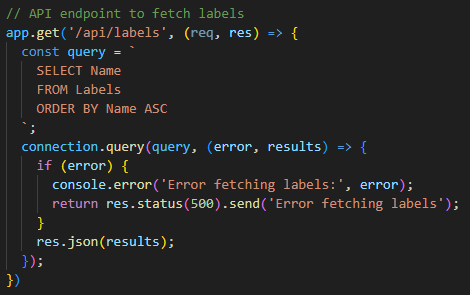
\includegraphics[width=\linewidth]{Queries/fetchLabels.png}
				\end{itemize}
				\item Fetching Genres
				\begin{itemize}
					\item 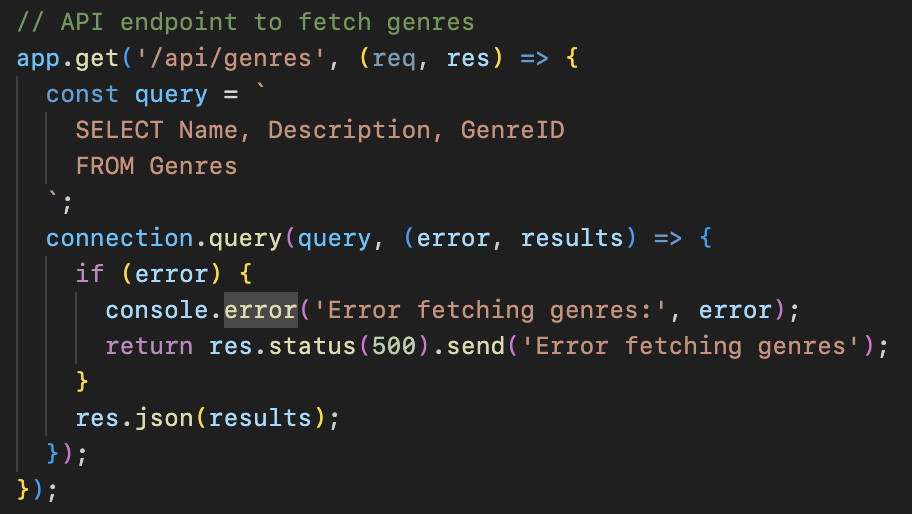
\includegraphics[width=\linewidth]{Queries/fetchGenres.png}
				\end{itemize}
				\item Fetching Subgenres by GenreID
				\begin{itemize}
					\item 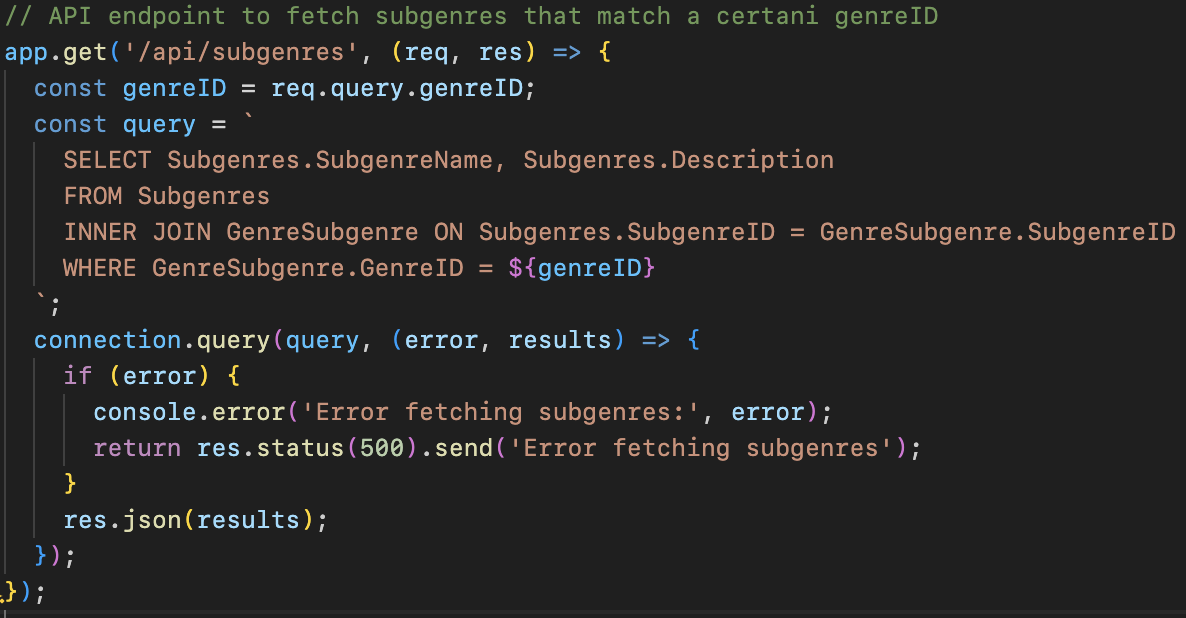
\includegraphics[width=\linewidth]{Queries/fetchSubgenresByGenreID.png}
				\end{itemize}
				\item Fetching Tracks by Artist Name
				\begin{itemize}
					\item 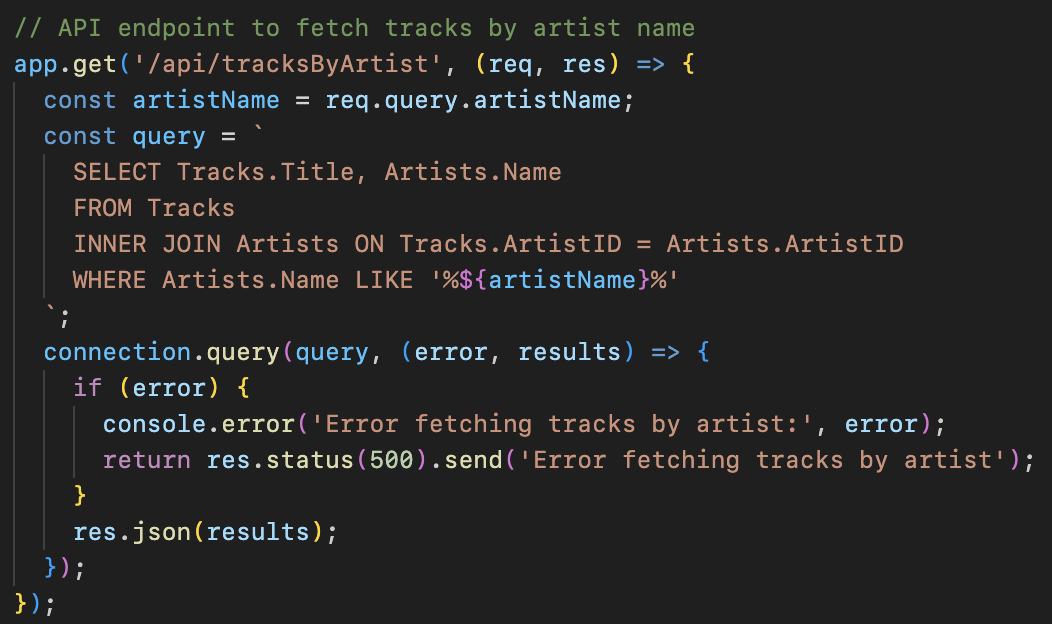
\includegraphics[width=\linewidth]{Queries/fetchTracksByArtistName.png}
				\end{itemize}
				\item Fetching Tracks by GenreID
				\begin{itemize}
					\item 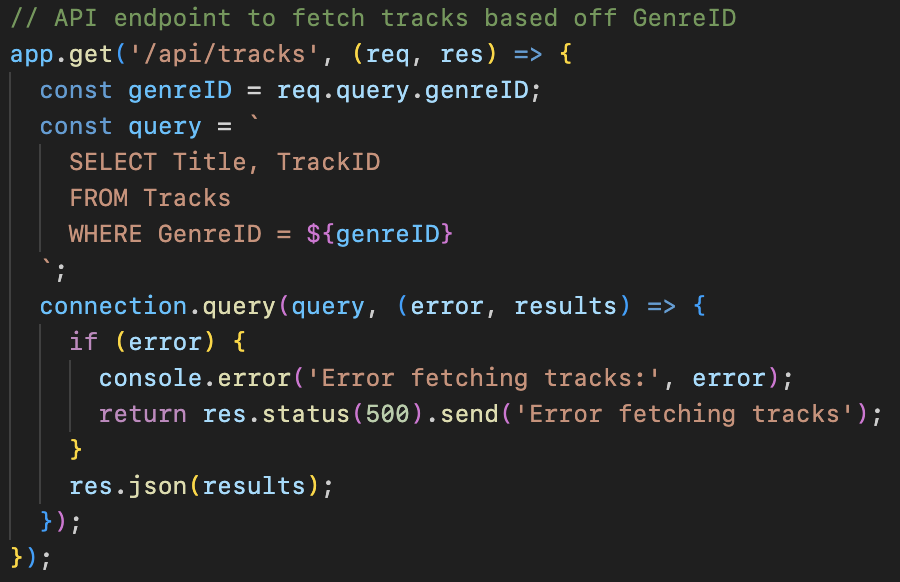
\includegraphics[width=\linewidth]{Queries/fetchTracksByGenreID.png}
				\end{itemize}
				\item Fetching Tracks by Title
				\begin{itemize}
					\item 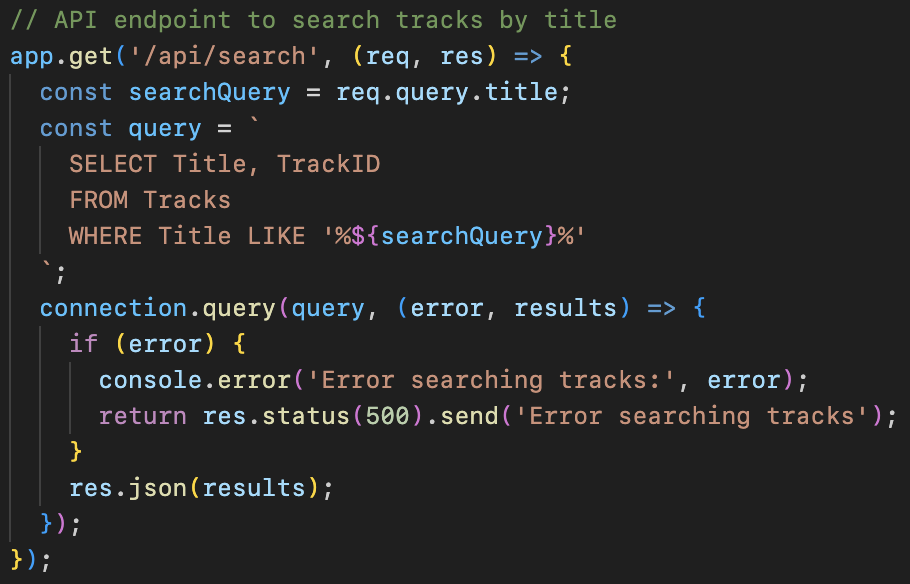
\includegraphics[width=\linewidth]{Queries/fetchTracksByTitle.png}
				\end{itemize}
    \end{itemize}

    \subsection{Python Data Scraping Scripts} Python scripts used for webscraping
    \begin{itemize}
        \item Main Scripts:
        \begin{itemize}
            \item $GenresScraper.py$ reads the data from our mostly manually generated JSON files containing genres and subgenres.
            \item $SetRaAlbumns.py$ imports the data cleaned by raScraper into our tables.
        \end{itemize}
        \item Scraper to collect data from resident advisor using GraphQL SQL Queries: $data/handling/scripts/raScraper$
        The python scripts use json files as templates for their queries.
        \begin{itemize}
            \item $album\_detail\_fetcher.py$ queries individiual album details
            \item $album\_fetcher.py$ queries lists of albums by genre.
            \item $album\_parser.py$ calls $album\_detail\_fetcher$ and $album\_fetcher$ scrapes all of the raw album data and then cleans the data to prepare it to add to our database
        \end{itemize}
    \end{itemize}

    \subsection{React App} 
    We built a react application to handle the front end which is responsible for the UI and asking the backend to communicate with our database
        \begin{itemize}
            \item Component Design
            All of our pages are built using the same general component design. Let's use albums as an example. There is an $albumPage.js$
            which renders the necessary $DataGrid.js$ components for each category matching the current filter. So if for example genre is the filter
            $AlbumPage.js$ creates a $DataGrid$ component for each genre. Each grid is loaded onto the page as a dropdown titled according to its category
            which when clicked reveals grid of $Album.js$ components. While all of the categories follow this same general structure, the filters and thus the queries used are slightly
            different for each category. 
            \item Search and Filter
            \begin{itemize}
                \item Search functionality allows user to query on any of the tables
                \item Filters vary by page allowing users to implement filters on the page they are on. To get entries matching specific parameters.
            \end{itemize}
            \item Genre page
            \begin{itemize}
                \item Displays genres as clickable dropdown menus to display subgenres belonging to a genre. Each subgenre shows its description when you hover over them.
            \end{itemize}
            \item Artists page
            \begin{itemize}
                \item Displays artists according to filters set by the user: options to filter by genre, year and label.
            \end{itemize}
            \item Mixes Page
            \begin{itemize}
                \item Displays DJ Mixes according to filters set by the user: options to filter by recommended, genre, year and label.
            \end{itemize}
            \item Albums Page
            \begin{itemize}
                \item Displays Albums according to filters set by the user: options to filter by recommended, genre, year and label.
            \end{itemize}
            \item Current Features
            \begin{itemize}
                \item Interactive pages built on Genres, Albums, Artists, Mixes and Labels tables.
                \item Filter and search by album, genre, artist, track, label, year and more.
            \end{itemize}
            \item Future Features
            \begin{itemize}
                \item Users database that allows users to follow other users as well as any other category within the database.
                \item Ability for users to add entries.
                \item Integration with streaming services to regularly and automatically update the database.
                \item Tree view to more easily visualize connections.
            \end{itemize}
        \end{itemize}
    \subsection{Testing}
        Although we did not implement any test suites or frameworks, if we were to continue the project we would. For the scale of our project we were able to test our queries using 
        the query interface on myPHP admin and then gradually test each component involved in a page in conjuction with the queries they used. We used debugging tools as well as including
        extensive error checking to make it easy to trace bugs in our code.


\section{Design Analysis}

\subsection{Constraints}

\subsubsection{Entity-Relationship Constraints}
\begin{itemize}
    \item Each artist, genre, subgenre, label, album, track and mix has a unique ID
\end{itemize}

\subsubsection{Referential Integrity Constraints}
\begin{itemize}
    \item All track, albums, and mixes have foreign keys which link them to genres, subgenres, artists, and labels.
    \item Subgenres have a foreign key to link them to genres
    \item Artists have foreign keys to link them to genres, subgenres, and labels.
\end{itemize}

\subsubsection{Consistency Constraints}
\begin{itemize}
    \item Any updates to an item that appears in multiple tables are reflect across all tables containing the item.
\end{itemize}

\subsection{Operations}

\subsubsection{Create Operations}
\begin{itemize}
    \item Add new artists, genres, labels, albums, tracks, and DJ mixes.
\end{itemize}

\subsubsection{Read Operations}
\begin{itemize}
    \item Retrieve information about users, artists, genres, labels, albums, tracks, and DJ mixes.
    \item Fetch lists of albums, tracks, and DJ mixes belonging to specific artists, genres, or labels.
    \item Fetch recommended Albums and Mixes.
\end{itemize}

\subsubsection{Update Operations}
\begin{itemize}
    \item Modify artist information, genre details, label information, album details, track details, and DJ mix details.
\end{itemize}

\subsubsection{Delete Operations}
\begin{itemize}
    \item Remove artists, genres, labels, albums, tracks, and DJ mixes from the database.
\end{itemize}

\subsubsection{Search Operations}
\begin{itemize}
    \item Search for users, artists, genres, labels, albums, tracks, and DJ mixes based on various criteria (e.g., name, genre, publication date).
    \item Perform advanced searches, such as finding tracks by artist or album name, or finding users with similar tastes.
\end{itemize}

\subsubsection{Aggregate Operations}
\begin{itemize}
    \item Aggregate data, such as counting the total number of albums, tracks, or DJ mixes in the database.
\end{itemize}

\subsubsection{Transactional Operations}
\begin{itemize}
    \item Execute transactions to maintain data consistency and integrity (e.g., updating multiple entities atomically).
\end{itemize}



\section{System Architecture}

\subsection{Original Entity Relationship Diagram}
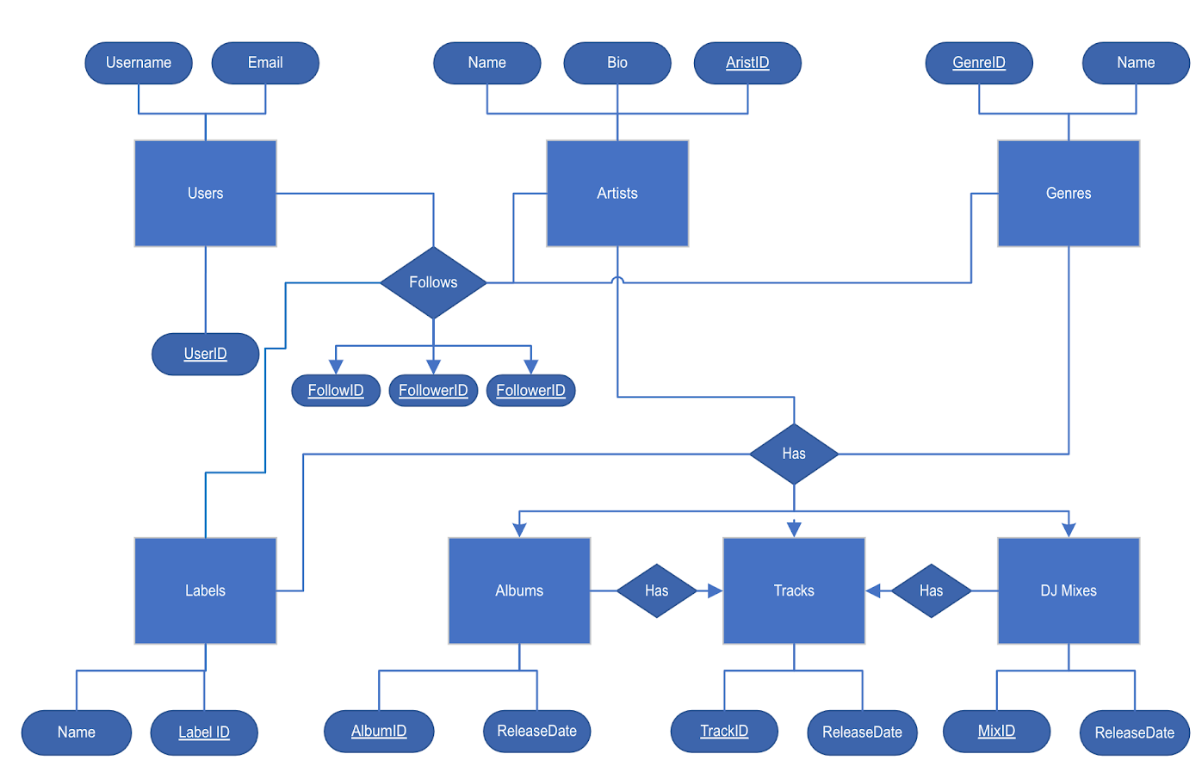
\includegraphics[width=\linewidth]{original_ER_diagram.png}

\subsection{Current Entity Relationship Diagram}
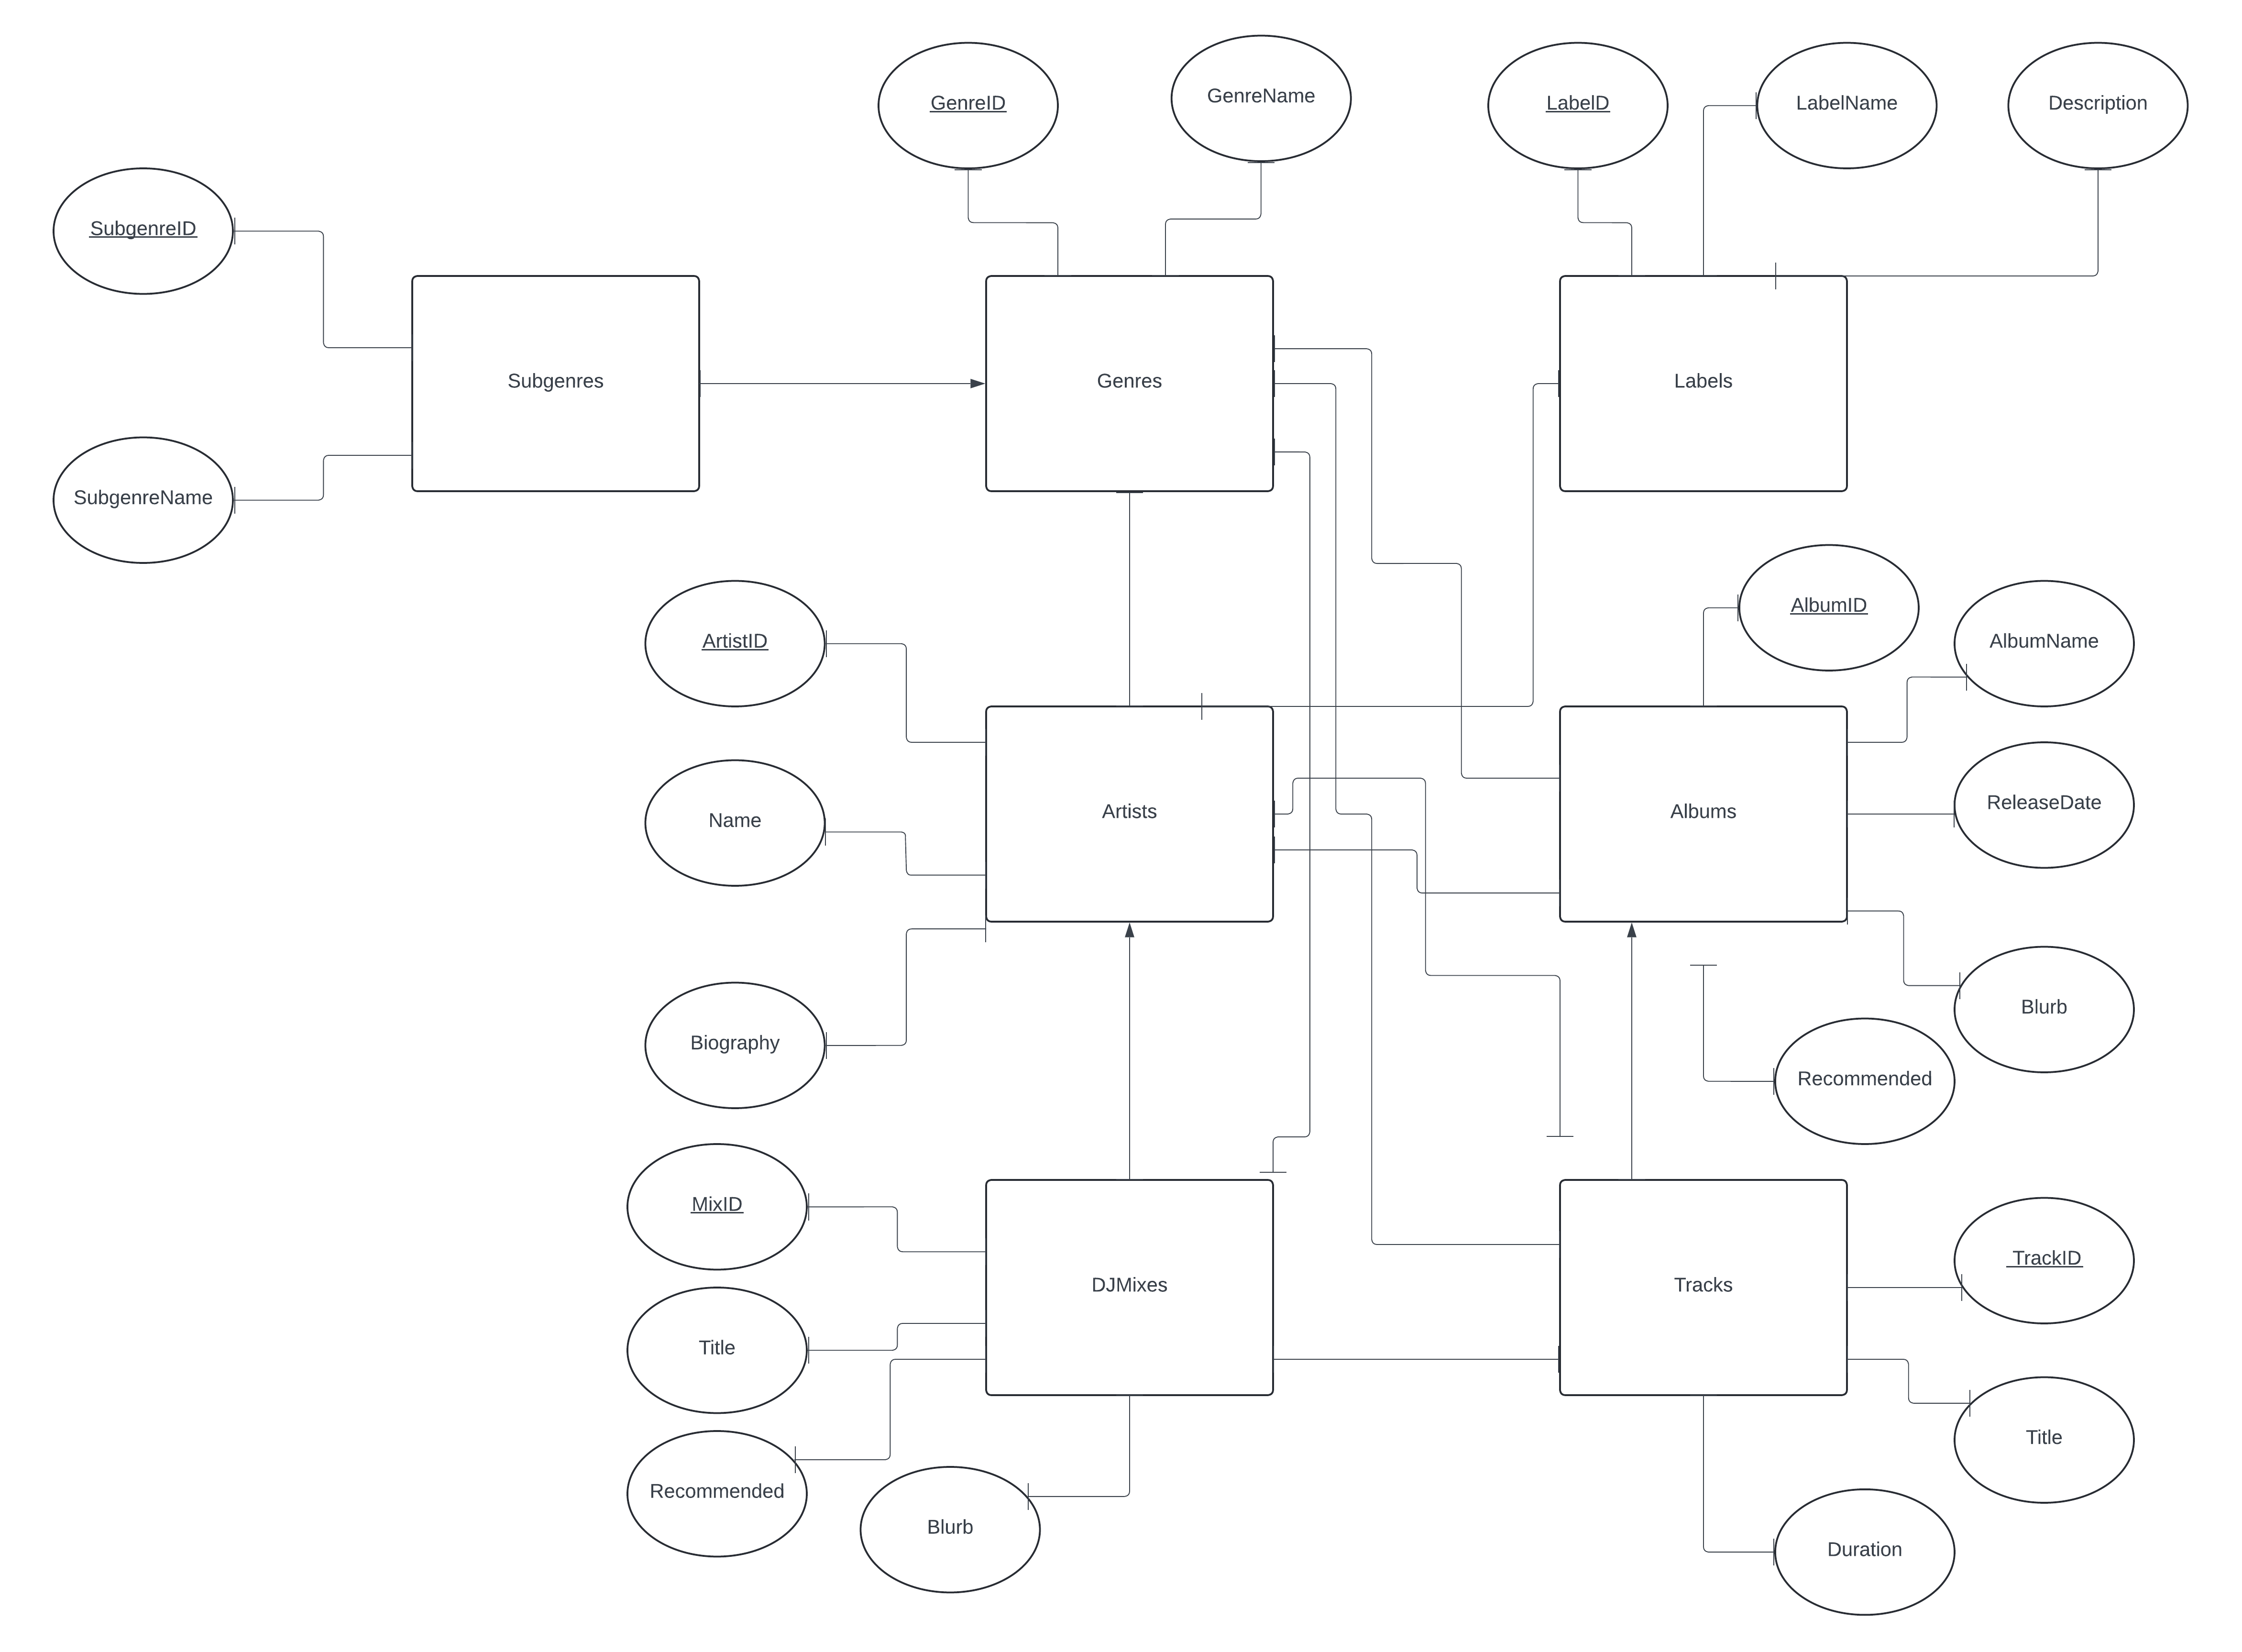
\includegraphics[width=\linewidth]{current_ER_diagram.png}

\subsection{Relational Schema}

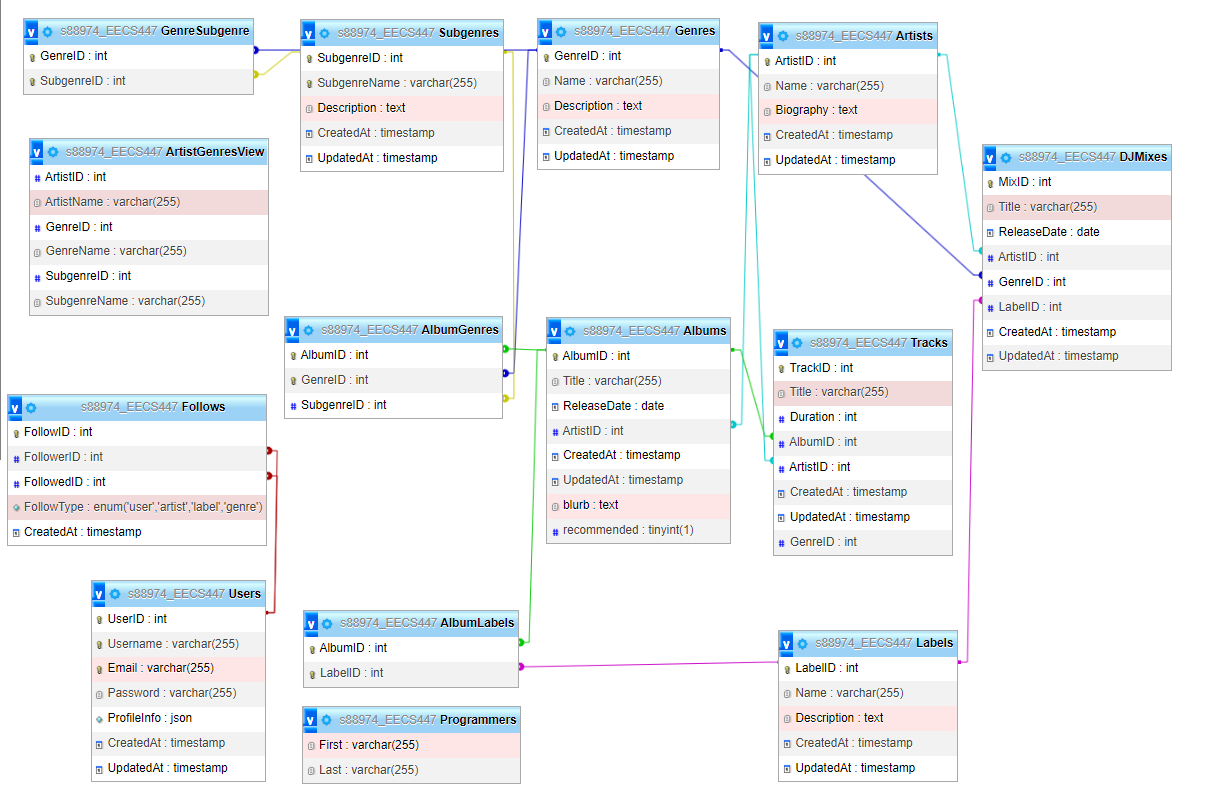
\includegraphics[width=\linewidth]{relational_schema.png}


\section{Project Log}
\subsection{General Responsibilities}
\begin{itemize}
    \item Zai Erb: 
    \begin{itemize}
        \item Wrote the reports
        \item Handled implementation of web scrapers
        \item Created SQL views and cleaned up database format after importing data 
        \item Handled designing the react application components and much of the styling
        \item Handled adding additional queries to the $api/server$  to get the filters for the various pages working.
    \end{itemize}

    \item Chinh Nguyen
    \begin{itemize}
        \item Implemented the server used in the backend to reference the database through phpMyAdmin
        \item Implemented and tested many of the queries used for searches and filters 
        \item Implemented a search page to test all of the searches/queries
    \end{itemize}

    \item Nicholas Nguyen:
    \begin{itemize}
        \item Assisted in research for building webscrapers
        \item Wrote the SQL to create the initial tables
        \item Helped to style the frontend and modify component behavior
        \item Created the project presentation
    \end{itemize}
\end{itemize}

\subsection{Specific Tasks}
The below tables more specifically detail what each group member did.
\pagebreak
\begin{table}[h!]
    \centering
    \resizebox{\textwidth}{!}{%
        \begin{tabular}{|l|l|l|}
            \hline
            \textbf{Contributor} & \textbf{Task} & \textbf{Time Spent} \\ \hline
            Zai Erb & Outlined and wrote first report & 2-3 hours \\ \hline
            Zai Erb, Nicholas Nguyen & Initialized React App and outlined component design & 2 hours \\ \hline
            Zai Erb & Experimented with webscraping for various sites & 5 hours \\ \hline
            Zai Erb, Chinh Nguyen, Nicholas Nguyen & Manually created JSON files for genres and subgenres & 4 hours \\ \hline
            Zai Erb, Chinh Nguyen & Implemented data cleaner to put JSON genre files into DB & 1 hour \\ \hline
            Zai Erb, Nicholas Nguyen & Attempted to implement 1001 tracklists scraper & 3 hours \\ \hline
            Zai Erb, Nicholas Nguyen & Updated styling & 2 hours \\ \hline
            Zai Erb & Modified database to make reference tables for foreign keys & 30 minutes \\ \hline
            Zai Erb & Implemented resident advisor scraper and data cleaner & 6+ hours \\ \hline
            Zai Erb & Updated backend and created references to display the front end according to filters on the page & \\ \hline
						Nicholas Nguyen & Began early front end work/design & 2 hours \\ \hline
						Nicholas Nguyen & Created initial SQL queries and attempted to implement them in the backend & 4 hours \\ \hline
						Nicholas Nguyen, Chinh Nguyen & Set up back end server and database for the project & 2 hours \\ \hline
						Nicholas Nguyen & Edited project video together, fixed audio for recordings. & 4 hours \\ \hline
						Chinh Nguyen, Nicholas Nguyen & Created project video slides and script & 2 hours \\ \hline
						Chinh Nguyen & Implemented and tested many of the queries used for searches and filters & 4 hours \\ \hline
        \end{tabular}
    }
    \caption{Contributions and Time Allocation}
    \label{tab:contributions}
\end{table}



\begin{table}[h!]
    \centering
    \resizebox{\textwidth}{!}{%
      \begin{tabular}{|c|c|c|}
\hline
Author & Date & Message \\
\hline
Zai Erb & 2024-05-06 & Added Report and Todo List \\
Zai Erb & 2024-05-06 & Added Report and Todo List \\
Zai Erb & 2024-05-02 & Added SQL views to simplify queries \\
Zai Erb & 2024-05-02 & Improved Scraper \\
Zai Erb & 2024-04-29 & Updated Styles \\
Zai Erb & 2024-04-29 & Added resident advisor scraper \\
Zai Erb & 2024-04-18 & styling \\
Chinh Nguyen & 2024-04-18 & Navigation bar now reflects the current page when site is refreshed \\
Zai Erb & 2024-04-18 & Search Styling \\
Zai Erb & 2024-04-17 & Styling \\
Chinh Nguyen & 2024-04-17 & STYLING! \\
Chinh Nguyen & 2024-04-17 & Fixed fetching tracks by artistName, doesn't have to be exact match now \\
Zai Erb & 2024-04-17 & Styling \\
Chinh Nguyen & 2024-04-17 & Cleaned up CSS, made scrollable, fixed naming \\
Chinh Nguyen & 2024-04-17 & Added search for tracks by artist name \\
Chinh Nguyen & 2024-04-17 & Added fetching tracks by artist name \\
Zai Erb & 2024-04-17 & Updated styling \\
Zai Erb & 2024-04-17 & Added GenreClick functionality for all pages. \\
Zai Erb & 2024-04-17 & Added all pages to sort items by Genre \\
Chinh Nguyen & 2024-04-17 & Implemented search artists by genreID \\
Chinh Nguyen & 2024-04-17 & Added 5th query with JOIN: Get artists based off GenreID \\
Chinh Nguyen & 2024-04-17 & Results Textarea \\
Zai Erb & 2024-04-17 & Genre Components \\
Chinh Nguyen & 2024-04-17 & Updated to include Search page \\
Chinh Nguyen & 2024-04-17 & Two new queries: Search Tracks based off genreID and title \\
Chinh Nguyen & 2024-04-17 & Basic Search Page \\
Zai Erb & 2024-04-17 & Added 1001 scraper. Not working \\
Chinh Nguyen & 2024-04-17 & Added more function \\
Chinh Nguyen & 2024-04-17 & Added Subgenre fetching using INNERJOIN on GenreID and SubgenreID \\
Chinh Nguyen & 2024-04-17 & Subgenre Fetch Function + Dropdown Divs \\
Chinh Nguyen & 2024-04-17 & Added query for Subgenre table: SubgenreName and Description \\
Chinh Nguyen & 2024-04-17 & Oops. Fixed reading of config.json \\
Nicholas Nguyen & 2024-04-17 & Fixed Genre alignment (along with other elements)

fixed weird redundancies too shared between each file.

added heart easter egg too because why not \\
Chinh Nguyen & 2024-04-17 & Necessary Packages Required, Added Localhost with Port 3001 as Proxy (IMPORTANT FOR BACKEND) \\
Chinh Nguyen & 2024-04-17 & Connected to the backend and displays "Genres" table with "Name" and "Description" column \\
Chinh Nguyen & 2024-04-17 & Working starter backend -- run with "node akiserver.js" in a second terminal, make sure that no other program is running port 3001 \\
Chinh Nguyen & 2024-04-17 & Password Leak -- Rotated Password / See Discord \\
Zai Erb & 2024-04-16 & Updated Genres Page - functional for presentation \\
Zai Erb & 2024-04-16 & Updated components and genre jsons \\
Zai Erb & 2024-04-16 & Updated JSON format \\
Zai Erb & 2024-04-16 & Fixed gitignore merge conflict \\
Zai Erb & 2024-04-16 & data changes \\
Zai Erb & 2024-04-16 & Data Changes \\
Nicholas Nguyen & 2024-04-16 & Furthered Front-End Design/Development \\
Nicholas Nguyen & 2024-04-15 & Add files via upload \\
Zai Erb & 2024-04-15 & Updated Scraper \\
Nicholas Nguyen & 2024-04-15 & Create .gitignore \\
Zai Erb & 2024-04-15 & Added raw data for genres in JSON files and added script to convert JSON into SQL tables \\
Zai Erb & 2024-04-03 & Added react project files \\
Zai Erb & 2024-04-03 & first commit \\
\hline
\end{tabular}
    }
    \caption{Git Commits}
    \label{tab:commits}
\end{table}


\end{document}
